\chapter{Posibile dezvolt\u ari}

\section{\^ Inv\u a\c tare prin \^ int\u arire}

\paragraph{}
\^ Inv\u a\c tarea prin \^ int\u arire sau Reinforcement learning (RL) reprezint\u a o arie machine learning inspirat\u a de psihologia comportamental\u a, a c\u arei principale preocup\u ari este cum poate un agent software s\u a \^ indeplineasc\u a anumite ac\c tiuni \^ intr-un mediu \^ inconjur\u ator astfel \^ inc\^ at s\u a maximizeze o r\u asplat\u a cumulativ\u a. Tipul acesta de \^ inv\u a\c tare difer\u a de metodele standard supervizate prin faptul c\u a sistemului nu \^ ii este prezentat niciodat\u a perechi de forma intrare-ie\c sire, precum nici rezolv\u ari ale unor ac\c tiuni suboptimale. Focusul principal este asupra performan\c tei on-line care presupune g\u asirea balan\c tei ideale \^ intre explorare (dob\^ andirea de cuno\c stin\c te noi) \c si exploatare (folosirea cuno\c stin\c telor curente). 

\paragraph{}
Modelul de baz\u a RL presupune:

\begin{itemize}
	\item Un set de st\u ari pentru mediu \c si agent \(S\)
	\item Un set de ac\c tiuni \(A\) ale agentului
	\item O politic\u a\footnote{policy} de tranzi\c tie de la st\u ari la ac\c tiuni
	\item Reguli care determin\u a r\u asplata scalar\u a imediat\u a a tranzi\c tiilor
	\item Reguli care descriu observa\c tiile agentului
\end{itemize}

\paragraph{}
Un agent RL interac\c tioneaz\u a cu mediul \^ in pa\c si de timpi discre\c ti. La fiecare pas \(t\), agentul prime\c ste o obsersva\c tie \(o_t\), care deobicei include o r\u asplat\u a \(r_t\). Apoi alege o ac\c tiune \(a_t\) din setul de ac\c tiuni posibile, care este trimis\u a mai departe c\u atre mediu. Mediul realizeaz\u a o tranzi\c tie c\u atre starea nou\u a \(s_{t+1}\), iar recompensa \(r_{t+1}\) asociat\u a cu tranzi\c tia \((s_t, a_t, s_{t+1})\) este determinat\u a (Figura 5.1).

\begin{figure}[H]
\centering
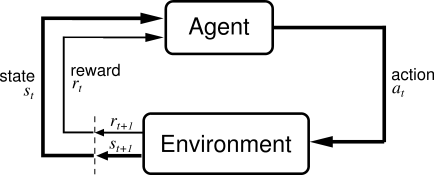
\includegraphics[width=0.6\textwidth]{reinforcement_learning}
\caption{Tranzi\c tia st\u arilor \^ in RL}
\end{figure}

\paragraph{}
Pentru a ac\c tiona aproape optim, agentul trebuie s\u a ia \^ in considerare dependen\c ta pe termen lung a ac\c tiunilor sale (s\u a maximizeze recompensa viitoare), chiar dac\u a r\u asplata imediat\u a este asociat\u a cu o valoare negativ\u a. Astfel, RL este potrivit pentru probleme unde exist\u a un compromis care include o recompens\u a \^ intre o dependen\c t\u a pe termen lung \c si una pe termen scurt. A fost aplicat cu succes \^ in diverse situa\c tii precum controlul automat de robo\c ti, telecomunica\c tii, jocuri ATARI \c si recent jocul GO.

\paragraph{}
Jiwei Li et al. propun \^ in articolul lor, Deep Reinforcement Learning for Dialogue Generation, utilizarea metodelor de RL pentru \^ inv\u a\c tare de limbaj. Plec\^ and de la aceea\c si arhitectur\u a HRED, descris\u a \^ in capitolul 3, se poate ca prin folosirea unor reguli euristice de determinare a recompensei, pe baza r\u aspunsurilor oferite de c\u atre chatbot, re\c teaua s\u a fie capabil\u a s\u a ofere r\u aspunsuri mai clare, contextuale \c si corect gramaticale. Astfel, articolul propune trei metode de recompens\u a pentru cuantificarea calit\u a\c tii unui r\u aspuns:

\begin{itemize}
	\item \(r_1\), care recompenseaz\u a modelul pentru r\u aspunsuri care nu fac parte dintr-un subset de r\u aspunsuri manual alese ca fiind monotone (I'm sorry, I don't know, Yes, No, etc.)
	\item \(r_2\), care recompenseaz\u a sistemul pentru nerepetarea aceluia\c si r\u aspuns consecutiv de mai multe ori la r\^ and
	\item \(r_3\), care recompenseaz\u a corectitudinea gramatical\u a \c si coeren\c ta r\u aspunsului
\end{itemize}


R\u asplata final\u a va fi o medie ponderat\u a \^ intre cele trei recompense:
\begin{center}
\(\lambda_1 r_1 + \lambda_2 r_2 + \lambda_3 r_3\)
\end{center}

unde \(\lambda_1 + \lambda_2 + \lambda_3 = 1\), iar \(\lambda_1 = 0.25, \lambda_2 = 0.25, \lambda_3 = 0.5\)

\paragraph{}
Folosind RL, autorii respectivi demonstreaz\u a c\u a rezultatele pot fi considerabil \^ imbun\u at\u a\c tite. De aceea, extinderea modelului curent pentru a folosi RL reprezint\u a una dintre principalele posibilele dezvolt\u ari dorite.

